\documentclass[10pt]{beamer}

\usetheme{m}

\usepackage{booktabs}
\usepackage[scale=2]{ccicons}

\usepackage{pgfplots}
\usepgfplotslibrary{dateplot}

\usepackage{graphicx}
\graphicspath{{img/}}

% strike through
\usepackage[normalem]{ulem}

% bitbucket icon
\usepackage{fontspec}
% fontawesome path
% \defaultfontfeatures{
%     Path = /usr/local/texlive/2015basic/texmf-dist/fonts/opentype/public/fontawesome/ }
\usepackage{fontawesome}

% color
\usepackage{xcolor}

\newcommand{\vfillall}{\vskip0pt plus 1filll}

\title{Efficient Gyro-Roller Based Rehabilitation Program For Stroke Patients}
%\subtitle{A modern beamer theme}
\date{}
\author{Tulakan Ruangrong}
\institute{AIMLAB - Biomedical Engineering - Mahidol University}
% \titlegraphic{\hfill\includegraphics[height=1.5cm]{logo/logo}}

\begin{document}

\maketitle

\begin{frame}
  \frametitle{Table of Contents}
  \setbeamertemplate{section in toc}[sections numbered]
  \tableofcontents[hideallsubsections]
\end{frame}

\section{Introduction}

\begin{frame}
  \frametitle{Stroke}
  	\hfill
	\newline
	\textbf{STROKE}
	\begin{itemize}
		\item Around \alert{\emph{20,000 deaths}} in Thailand every year.
		\item Major cause of paralytic.
	\end{itemize}
	\begin{figure}[h]
	\centering
	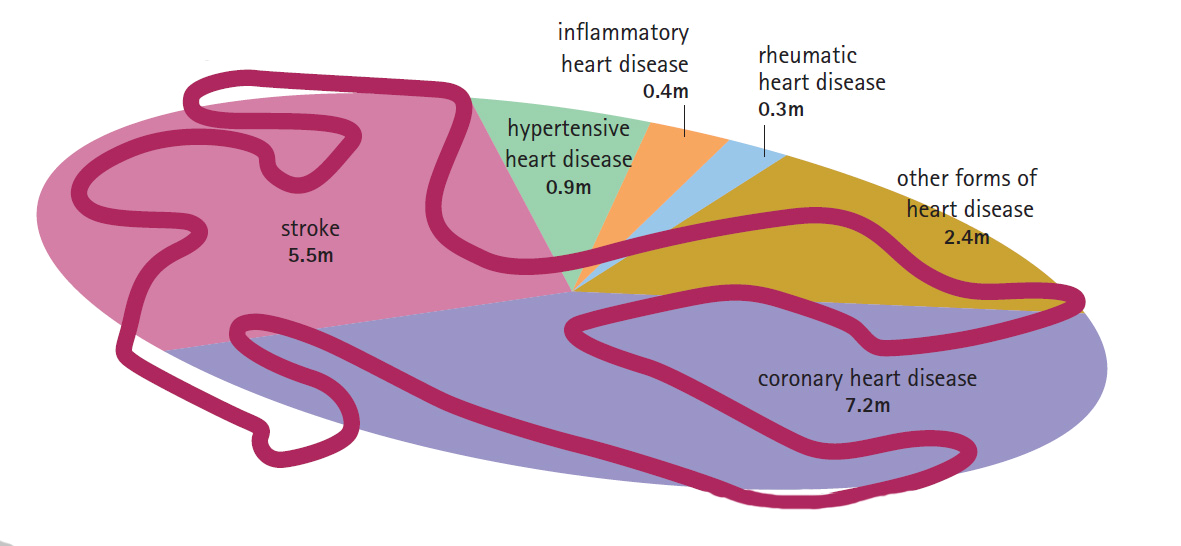
\includegraphics[width=0.7\textwidth]{stat}
	\caption{Global deaths from Cardiovascular disease}
	\end{figure}
\end{frame}

\begin{frame}{Rehabilitation}
	\textbf{REHABILITATION}
	\begin{itemize}
		\item \alert<1>{Neural plasticity}
		\item \alert<2>{Most of commercial devices are very expensive}
		\item \alert<3>{Strict and repetitive process}
		\item \alert<4>{Easy to be motiveless and bored}
	\end{itemize}
	\hfill
	\hfill
	\begin{center}
		\alert<5>{\uppercase{\Large{\emph{\textbf{Combination between virtual reality and rehabilitation techniques}}}}}
	\end{center}
\end{frame}

\begin{frame}{Gyro-Roller}
	\begin{columns}[c]
		\column{0.65\textwidth}
		\begin{figure}[h]
			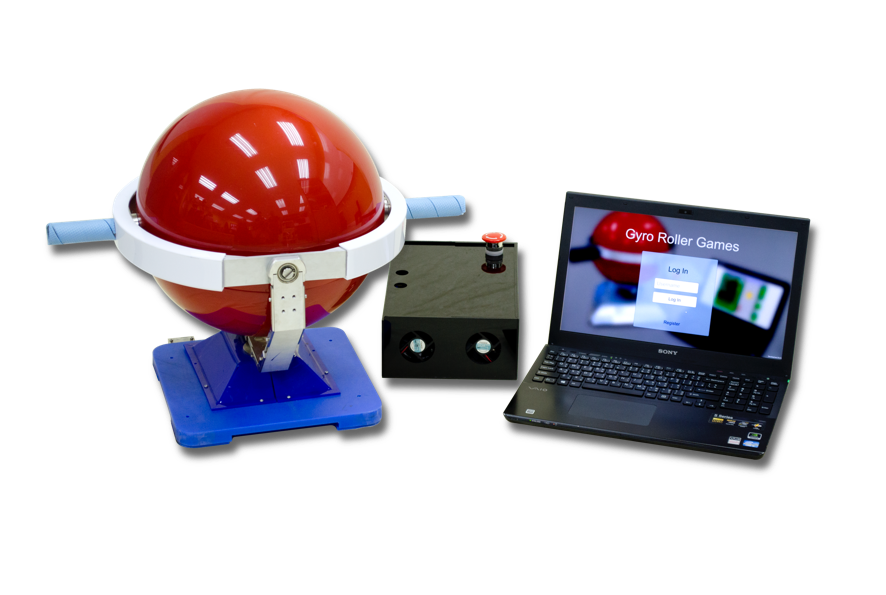
\includegraphics[width=\textwidth]{gyrosys}
			\caption{Gyro-Roller System}
		\end{figure}
		\column{0.35\textwidth}
		\begin{figure}[h]
			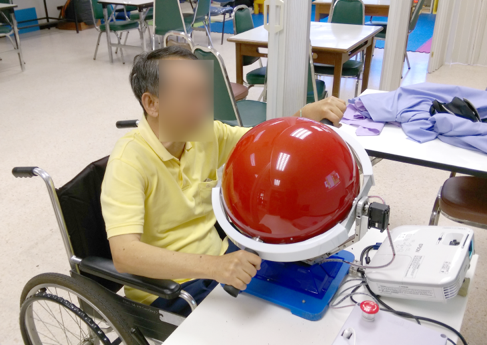
\includegraphics[width=\textwidth]{patient1}
			\newline
			\break
			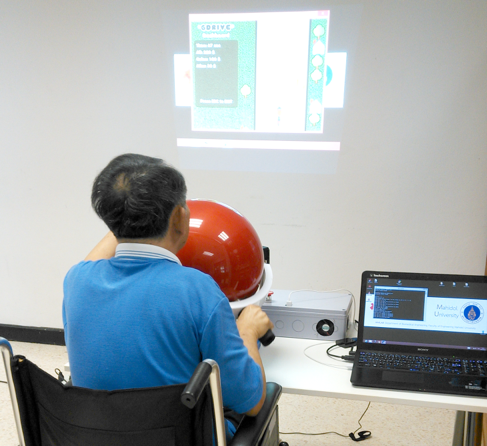
\includegraphics[width=\textwidth]{patient2}
			\caption{With patients}
		\end{figure}
	\end{columns}
\end{frame}

\begin{frame}{Gyro-Roller}
	\textbf{Difference between 2nd and 3rd version}
	\break
	\begin{columns}[c]
		\column{0.5\textwidth}
		\begin{figure}
			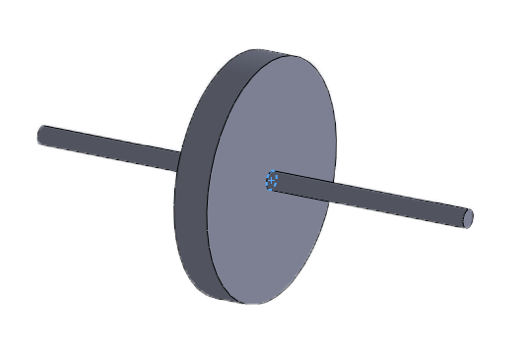
\includegraphics[width=\textwidth]{wheel_ver2}
			\caption{Version 2 wheel}
		\end{figure}
		\column{0.5\textwidth}
		\begin{figure}
			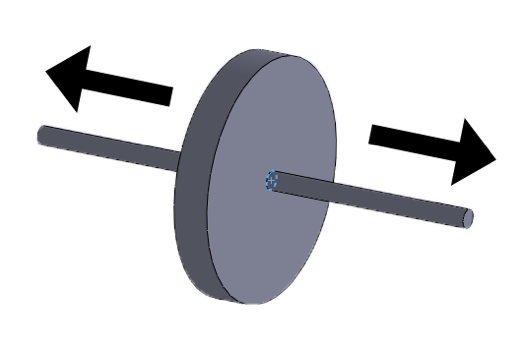
\includegraphics[width=\textwidth]{wheel_ver3}
			\caption{Version 3 wheel}
		\end{figure}
	\end{columns}
\end{frame}

\begin{frame}{Thesis Objectives}
	\hfill
	\begin{itemize}
		\large{
		\item Game Design
		\item Virtual Reality based Gyro-Roller system
		\item Clinical Trial
		}
	\end{itemize}
	\begin{figure}[h]
		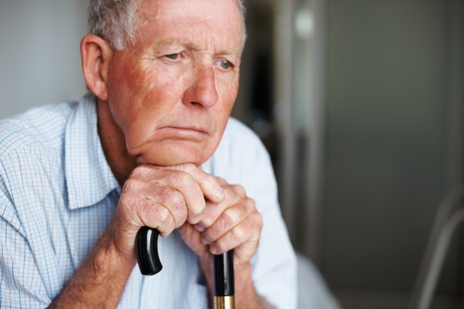
\includegraphics[width=0.4\textwidth]{elder}
		\,\,\,\,
		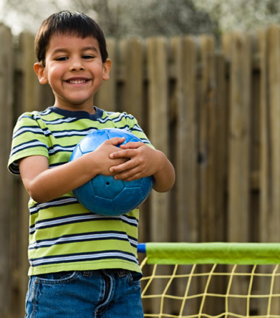
\includegraphics[width=0.3\textwidth]{child}
	\end{figure}
\end{frame}

\begin{frame}{Thesis Scopes}
	\begin{itemize}
		\large{\alert<1>{\item Develop 3 different games with active \& passive modes including several levels and log file.}
		\alert<2>{\item Find out how effective of the Gyro-Roller version 3 over version 2.}
		\alert<3>{\item Collect the data of 20 subjects for at least 2 months.}}
	\end{itemize}
\end{frame}

\section{Previous Works}
% new command used - creating strikethrough function
% \newcommand{\sttr}[1]{\rlap{\rule[0.5ex]{6em}{0.1ex}}\text{#1}}


\begin{frame}{Problem Solved}
	\large \textbf{Mechanic}
	\normalsize
	\begin{itemize}
		\item \sout{Fix pulley belt tension}
		\item \sout{Fix handle bar alignment}
		\item \sout{Wiring servomotor -> tuning goal position}
	\end{itemize}
	
	\large \textbf{Software}
	\normalsize
	\begin{itemize}
		\item \sout{Write new Arduino sketch to control DC motor}
	\end{itemize}
\end{frame}

\begin{frame}{Game Development}
	\vfillall
	\large \textbf{Game pages – integrated}
	\begin{itemize}
		\item Login
		\item Registration
		\item Game Selector
		\item Calibration – with motor connected
		\item EMG collection game 
		\item Space shooting game – \alert{being integrated}
	\end{itemize}
	\vfillall
	\centering \footnotesize \# This project is tracked using \emph{git} with \,{\color{blue!52!cyan}\faBitbucket \,Bitbucket}
	\smallskip
\end{frame}
%--- Next Frame ---%

\section{Present Works}
	\begin{frame}{Present Works}
	\begin{columns}[t]
		\column{0.5\textwidth}
			\large \textbf{Literature Review}
			\normalsize
			\begin{itemize}
				\item Cognitive rehabilitation
				\item Serious game for rehabilitation \newline\newline 
			\end{itemize}

			\large \textbf {Game Development}
			\normalsize
			\begin{itemize}
				\item Add mode to control mass movement
				\item Design and create cognitive based games
			\end{itemize}
		\column{0.5\textwidth}
			\large \textbf{EMG Analysis}
			\normalsize
			\begin{itemize}
				\item Figure difference between mass to the left-right
				\item Apply information to the game \newline
			\end{itemize}
			\large \textbf{Mechanic}
			\normalsize
			\begin{itemize}
				\item Sent device back to fix problems
			\end{itemize}
	\end{columns}		
	\end{frame}
	
	\begin{frame}{Literature Review}
		\begin{figure}[h]
			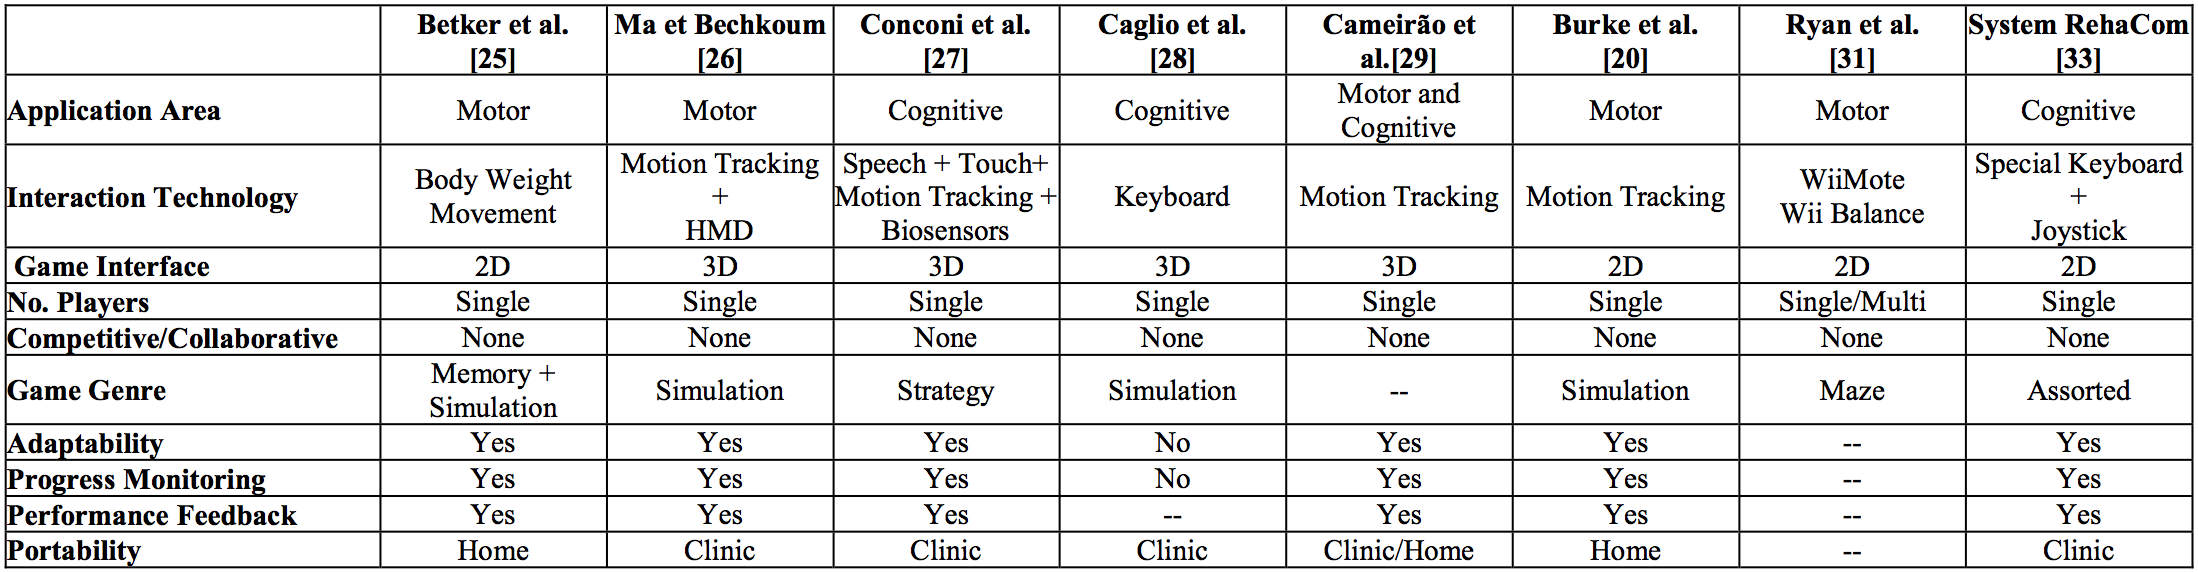
\includegraphics[width=\textwidth]{serious_game_table.png}
			\caption{Classification and comparison of rehabilitation serious games}
		\end{figure}
	\end{frame}
	
	\begin{frame}{Game Development}
		\large \textbf{Add mode to control mass movement}
		\normalsize
		\begin{itemize}
			\item Able to move automatically
			\item But not able to control movement speed for now
		\end{itemize}
		\large \textbf{What to do}
		\normalsize
		\begin{itemize}
			\item Add ability to control speed into library
			\item Write some of the basic games that are cognitive related (EMG results would be applied afterward)
		\end{itemize}
	\end{frame}
	
	\begin{frame}{EMG Analysis}
		\large \textbf{What to do}
		\normalsize
		\begin{itemize}
			\item Design proper experiment to investigate difference during wheel movement
			\item Wait for the Gyro-Roller to come back from factory
		\end{itemize}
	\end{frame}
	
	\begin{frame}{Mechanic}
		\large \textbf{Problem}
		\normalsize
		\begin{itemize}
			\item Can't contact manufacturer
		\end{itemize}
		\large \textbf{What to do}
		\normalsize
		\begin{itemize}
			\item Keep contacting
			\item Order cover parts (acrylic dome)
		\end{itemize}
	\end{frame}
	%--- Next Frame ---%
%--- Next Frame ---%
	
	
	
	









% \begin{frame}[fragile]
%   \frametitle{Typography}
%       \begin{verbatim}The theme provides sensible defaults to
% \emph{emphasize} text, \alert{accent} parts
% or show \textbf{bold} results.\end{verbatim}
%
%   \begin{center}becomes\end{center}
%
%   The theme provides sensible defaults to \emph{emphasize} text,
%   \alert{accent} parts or show \textbf{bold} results.
% \end{frame}
% \begin{frame}{Lists}
%   \begin{columns}[T,onlytextwidth]
%     \column{0.33\textwidth}
%       Items
%       \begin{itemize}
%         \item Milk \item Eggs \item Potatos
%       \end{itemize}
%
%     \column{0.33\textwidth}
%       Enumerations
%       \begin{enumerate}
%         \item First, \item Second and \item Last.
%       \end{enumerate}
%
%     \column{0.33\textwidth}
%       Descriptions
%       \begin{description}
%         \item[PowerPoint] Meeh. \item[Beamer] Yeeeha.
%       \end{description}
%   \end{columns}
% \end{frame}
% \begin{frame}{Animation}
%   \begin{itemize}[<+- | alert@+>]
%     \item \alert<4>{This is\only<4>{ really} important}
%     \item Now this
%     \item And now this
%   \end{itemize}
% \end{frame}
% \begin{frame}{Figures}
%   \begin{figure}
%     \newcounter{density}
%     \setcounter{density}{20}
%     \begin{tikzpicture}
%       \def\couleur{alerted text.fg}
%       \path[coordinate] (0,0)  coordinate(A)
%                   ++( 90:5cm) coordinate(B)
%                   ++(0:5cm) coordinate(C)
%                   ++(-90:5cm) coordinate(D);
%       \draw[fill=\couleur!\thedensity] (A) -- (B) -- (C) --(D) -- cycle;
%       \foreach \x in {1,...,40}{%
%           \pgfmathsetcounter{density}{\thedensity+20}
%           \setcounter{density}{\thedensity}
%           \path[coordinate] coordinate(X) at (A){};
%           \path[coordinate] (A) -- (B) coordinate[pos=.10](A)
%                               -- (C) coordinate[pos=.10](B)
%                               -- (D) coordinate[pos=.10](C)
%                               -- (X) coordinate[pos=.10](D);
%           \draw[fill=\couleur!\thedensity] (A)--(B)--(C)-- (D) -- cycle;
%       }
%     \end{tikzpicture}
%     \caption{Rotated square from
%     \href{http://www.texample.net/tikz/examples/rotated-polygons/}{texample.net}.}
%   \end{figure}
% \end{frame}
% \begin{frame}{Tables}
%   \begin{table}
%     \caption{Largest cities in the world (source: Wikipedia)}
%     \begin{tabular}{lr}
%       \toprule
%       City & Population\\
%       \midrule
%       Mexico City & 20,116,842\\
%       Shanghai & 19,210,000\\
%       Peking & 15,796,450\\
%       Istanbul & 14,160,467\\
%       \bottomrule
%     \end{tabular}
%   \end{table}
% \end{frame}
% \begin{frame}{Blocks}
%   Three different block environments are pre-defined and may be styled with an
%   optional background color.
%
%   \begin{columns}[T,onlytextwidth]
%     \column{0.5\textwidth}
%       \begin{block}{Default}
%         Block content.
%       \end{block}
%
%       \begin{alertblock}{Alert}
%         Block content.
%       \end{alertblock}
%
%       \begin{exampleblock}{Example}
%         Block content.
%       \end{exampleblock}
%
%     \column{0.5\textwidth}
%
%       \metroset{block=fill}
%
%       \begin{block}{Default}
%         Block content.
%       \end{block}
%
%       \begin{alertblock}{Alert}
%         Block content.
%       \end{alertblock}
%
%       \begin{exampleblock}{Example}
%         Block content.
%       \end{exampleblock}
%
%   \end{columns}
% \end{frame}
% \begin{frame}{Math}
%   \begin{equation*}
%     e = \lim_{n\to \infty} \left(1 + \frac{1}{(n+1)^n}\right)^n
%   \end{equation*}
% \end{frame}
% \begin{frame}{Line plots}
%   \begin{figure}
%     \begin{tikzpicture}
%       \begin{axis}[
%         mlineplot,
%         width=0.9\textwidth,
%         height=6cm,
%       ]
%
%         \addplot {sin(deg(x))};
%         \addplot+[samples=100] {sin(deg(2*x))};
%
%       \end{axis}
%     \end{tikzpicture}
%   \end{figure}
% \end{frame}
% \begin{frame}{Bar charts}
%   \begin{figure}
%     \begin{tikzpicture}
%       \begin{axis}[
%         mbarplot,
%         xlabel={Foo},
%         ylabel={Bar},
%         width=0.9\textwidth,
%         height=6cm,
%       ]
%
%       \addplot plot coordinates {(1, 20) (2, 25) (3, 22.4) (4, 12.4)};
%       \addplot plot coordinates {(1, 18) (2, 24) (3, 23.5) (4, 13.2)};
%       \addplot plot coordinates {(1, 10) (2, 19) (3, 25) (4, 15.2)};
%
%       \legend{lorem, ipsum, dolor}
%
%       \end{axis}
%     \end{tikzpicture}
%   \end{figure}
% \end{frame}
% \begin{frame}{Quotes}
%   \begin{quote}
%     Veni, Vidi, Vici
%   \end{quote}
% \end{frame}
%
% \begin{frame}{References}
%   % Some references to showcase [allowframebreaks] \cite{knuth92,ConcreteMath,Simpson,Er01,greenwade93}
% \end{frame}
%
% \section{Conclusion}
%
% \begin{frame}{Summary}
%
%   Get the source of this theme and the demo presentation from
%
%   \begin{center}\url{github.com/matze/mtheme}\end{center}
%
%   The theme \emph{itself} is licensed under a
%   \href{http://creativecommons.org/licenses/by-sa/4.0/}{Creative Commons
%   Attribution-ShareAlike 4.0 International License}.
%
%   \begin{center}\ccbysa\end{center}
%
% \end{frame}

\plain{END}

% \begin{frame}[allowframebreaks]
%
%   \frametitle{References}
%
%   \bibliography{demo}
%   \bibliographystyle{abbrv}
%
% \end{frame}

\end{document}
